% http://www.ctan.org/tex-archive/macros/latex/contrib/beamer/examples
% http://latex.artikel-namsu.de/english/beamer-examples.html

\documentclass{beamer}
\usepackage{amsmath}
\usepackage{amssymb}
\usepackage{bm}
\usepackage{fancybox, graphicx}
\usepackage{listings}
\usepackage{tikz} % Diagrams
\usepackage{color}

\iffalse
\lstdefinestyle{customc}{
  belowcaptionskip=1\baselineskip,
  breaklines=true,
  %frame=L,
  xleftmargin=\parindent,
  language=bash,
  showstringspaces=false,
  basicstyle=\footnotesize\ttfamily,
  keywordstyle=\bfseries\color{green!40!black},
  commentstyle=\itshape\color{purple!40!black},
  identifierstyle=\color{blue},
  stringstyle=\color{orange},
  deletekeywords={login}, % Needed to prevent spurious colouring of `login' where it appears in `splinter-login'.
}
\lstset{style=customc}
\fi
\lstset{language=Python}



\usetheme{boxes}
\usecolortheme{beaver}


\title[IT Workshops] % (optional, use only with long paper titles)
{Introduction to IT for UCL Astrophysicists}

\author{L.~Whiteway, T.~Wilson, W.~Jennings, E.~Edmondson, L.~Lucie-Smith}

\institute[UCL]
{
  Department of Physics and Astronomy\\
  University College London
}
\date[IT 2016]
{13 \& 20 October 2016}

\subject{IT}

\begin{document}

\frame{\titlepage}

\section{Introduction}

\begin{frame}{Where to find this presentation}
  \begin{block}{}
    \url{http://tinyurl/hhndmla}
  \end{block}
\end{frame}


\begin{frame}{Overall goals of presentation}
  \begin{itemize}
    \item What software you might find useful
    \item Where to get more information (UCL courses, web, etc.)
    \item UCL-specific information (e.g. login details)
    \item Some hands-on work
  \end{itemize}
\end{frame}

\begin{frame}{Specific contents}

  \begin{block}{13 October:}
    \begin{itemize}
      \item Accessing Astrophysics group machines
      \item Using the Linux console
      \item Basics of Python
    \end{itemize}
  \end{block}
  
  \begin{block}{20 October:}
    \begin{itemize}
    \item Commonly used programs (LaTeX, DS9, IRAF,...)
    \item Using High-Performance Computing (HPC) machines
    \item HPC best practices
    \end{itemize}
  \end{block}
  
  \begin{block}{A further session on 27 October will cover machine learning using Python.}
  \end{block}

\end{frame}

\begin{frame}{Information on the Web}
  \begin{block}{Astrophysics Wiki}
    \url{https://wiki.ucl.ac.uk/display/PhysAstAstPhysGrp/Main+Page}
    This Wiki is freely viewable and editable by all members of the department. Please use it to record information that you think will be useful to others (including your future self). Be bold!
  \end{block}

  \begin{block}{UCL Research Computing Platforms}
    \url{https://wiki.rc.ucl.ac.uk/wiki/Main_Page}
  \end{block}
  
  \begin{block}{Stack Overflow}
    \url{http://stackoverflow.com/}
  \end{block}
  
\end{frame}



\begin{frame}{Computing Environment for Astrophysics}
  \begin{itemize}
  \item Large datasets requiring substantial processing followed by sophisticated statistical analysis
  \item Calculations often done on specialised `high-performance computing' (HPC) machines having large filesystems and large RAM; calculations are often broken into pieces that can be run simultaneously (`in parallel') across many processors.
  \item Much useful software is made freely available within the community. Software quality is usually high; documentation quality is more variable.
  \item Many users write their own software.
  \end{itemize}
\end{frame}

\begin{frame}{Local Computing Environment}
  \begin{block}{You will have your own local machine, which might be:}
    \begin{itemize}
      \item PC (Windows)
      \item Mac
      \item Linux
    \end{itemize}
  \end{block}
  \begin{block}{Also there are shared Linux machines:}
    \begin{itemize}
      \item General purpose Astrophysics server available from outside UCL: \alert{\texttt{zuserver1}}
      \item UCL Cosmology HPC cluster: \alert{\texttt{splinter}}
      \item Other UCL HPC clusters: \alert{\texttt{Grace}}, \alert{\texttt{Legion}} and \alert{\texttt{Emerald}}
      \item National HPC cluster: \alert{\texttt{DiRAC}}
    \end{itemize}
  \end{block}
\end{frame}

\begin{frame}{Work patterns}
  \begin{block}{Several work patterns are possible:}
    \begin{itemize}
      \item Write and test a program on your local machine; use the local machine to remotely connect to \texttt{splinter}; upload the program to \texttt{splinter} and run it there;
      \item Or do all your work locally (requires small data sets);
      \item Or use the local machine to remotely connect to \texttt{splinter} and do all your work there.
    \end{itemize}
  \end{block}
\end{frame}

\begin{frame}{Remote connections}
  \begin{block}{How to connect to a shared machine}
    \begin{itemize}
      \item Windows PC: use PuTTY;
      \item Mac: go to the Terminal window and use \texttt{ssh};
      \item Linux machine: go to the Terminal window and use \texttt{ssh}.
    \end{itemize}
  \end{block}
  \begin{block}{Visibility}
    If you are not on the UCL network then you cannot connect to \texttt{splinter} directly; instead you must go via \texttt{zuserver1}.
  \end{block}
\end{frame}


\begin{frame}{Two methods for accessing splinter}
  \begin{figure}
    \begin{center}
      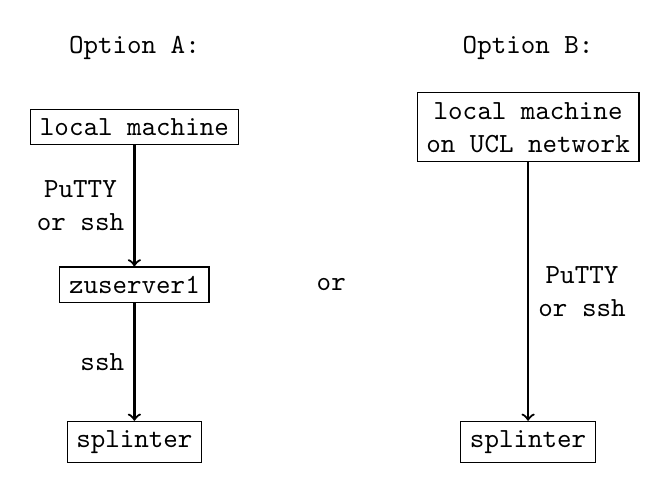
\begin{tikzpicture}[font=\ttfamily]
        \node at (-2.5, 6) {Option A:};
        \node at (2.5, 6) {Option B:};
        \node (LM1) at (-2.5,5) [rectangle,draw] {local machine};
        \node (Z) at (-2.5,3) [rectangle,draw] {zuserver1};
        \node (S1) at (-2.5,1) [rectangle,draw] {splinter};
        \node (LM2) at (2.5,5) [rectangle,draw,align=center] {local machine \\ on UCL network};
        \node (S2) at (2.5,1) [rectangle,draw] {splinter};
        \node at (0,3) {or};
        \draw [->,thick] (LM1.south) -- (Z.north) node [midway,left,align=center] {PuTTY \\ or ssh};
        \draw [->,thick] (Z.south) -- (S1.north) node [midway,left] {ssh};
        \draw [->,thick] (LM2.south) -- (S2.north) node [midway,right,align=center] {PuTTY \\ or ssh};
      \end{tikzpicture}
    \end{center}
  \end{figure}
\end{frame}

\begin{frame}{Accessing remote machines}
  \begin{block}{Credentials}
    \begin{itemize}
      \item You will need a \textit{username} and \textit{password} for \texttt{splinter} (and, if you are using Option A, for \texttt{zuserver1} as well).
      \item If you do not have these already then we can give guest credentials to be used during this course.
    \end{itemize}
  \end{block}
  \begin{block}{The full names of the servers are:}
    \begin{itemize}
      \item \texttt{zuserver1.star.ucl.ac.uk}
      \item \texttt{splinter-login.star.ucl.ac.uk}
    \end{itemize}
  \end{block}
\end{frame}


\begin{frame}{Using PuTTY for remote connections from Windows}
  \begin{itemize}
    \item If you don't have PuTTY you can download it from \url{http://www.putty.org/}.
    \item On the `Connection/SSH/X11' tab, click on `enable X11 forwarding' and set `X display location' to `localhost:0' - this is necessary for handling graphical output.
    \item On the Session tab, set the Host Name as appropriate: \texttt{zuserver1.star.ucl.ac.uk} (Option A) or \texttt{splinter-login.star.ucl.ac.uk} (Option B).
  \end{itemize}
\end{frame}

\begin{frame}{Using ssh for remote connections from Mac and Linux}
  \begin{itemize}
    \item Syntax: \alert{\texttt{ssh -YC username@servername}}
    \item The `Y' option is necessary for handling graphical output.
  \end{itemize}
\end{frame}

\begin{frame}{X-Windows client}
  \begin{itemize}
    \item If the remote program that you are running produces graphical output, then you must have a program (an `X-Windows client') running on your local machine to display this graphical output.
    \item On Windows you can use XMing (\url{https://sourceforge.net/projects/xming/}) or Exceed (available on the UCL Desktop).
    \item On Mac you can use XQuartz.
    \item On Linux you can sit back and relax as the graphical interface is an X-server.
  \end{itemize}
\end{frame}


\section{Linux}

\begin{frame}{Linux: Command shell}
  \begin{itemize}
    \item{In Linux you will use a `command shell'.}
    \item{This is a text-based environment in which you type commands and receive text output.}
    \item{Not GUI! Reflects the hardware limitations current when Unix was created. Low-tech and reliable e.g. for remote access.}
    \item{Various command shell programs are used: \texttt{bash}, \texttt{csh}, \texttt{tcsh}, etc. To see which one you are using, call \texttt{echo \$0}.}
   \end{itemize}
\end{frame}

\begin{frame}{Linux: Directory structure}
  \begin{itemize}
    \item{Everything is organised around files (which may be data files or program files i.e. instructions to be executed).}
    \item{Files live in directories. There is a hierarchical tree structure of directories.}
    \item{Sample file name: \texttt{/share/splinter/ucapwhi/des/foo.txt}}
    \item{Note use of slash `/', not backslash `\textbackslash' as in Windows.}
    \item{Case sensitivity: `Foo' and `foo' are different strings.}
  \end{itemize}
\end{frame}

\begin{frame}{Linux: Special symbols for directories}
  \begin{table}[ht]
    \centering
    \begin{tabular}{c l}
      \\ [-2ex]
      Symbol & Meaning \\ [.5ex]
      \hline \\ [-2ex]
      / & Top of the directory tree (the root directory) \\
      . & Current directory \\
      .. & Parent of the current directory \\
      \textasciitilde & User's `home' directory
    \end{tabular}
  \end{table}

    \begin{block}{}
  
    \end{block}
    \begin{block}{}
       Remember, \texttt{TAB} is your friend.
    \end{block}



\end{frame}


\begin{frame}{Linux: Environment variables}
  \begin{itemize}
    \item The operating system maintains a global namespace of `environment variables' to store configuration information.
    \item Use \alert{\texttt{printenv}} (in tcsh) or \alert{\texttt{set}} (in bash) to see all environment variables; use \alert{\texttt{echo \$<variable\_name>}} to see the value of one environment variable (e.g. \alert{\texttt{echo \$PATH}}).
    \item Use \alert{\texttt{setenv FOO my\_string}} (in tcsh) or \alert{\texttt{export \$FOO=`my\_string'}} (in bash) to set \texttt{FOO}.
    \item Variables \texttt{PATH} and \texttt{PYTHONPATH} are used frequently (to maintain lists of directories in which to search for executable programs and Python modules, respectively).
    \item Linux has no equivalent of the Windows Registry; configuration is done via the directory structure and the environment variables.
  \end{itemize}
\end{frame}



\begin{frame}{Linux: Structure of commands}
  \begin{block}{Structure}
    \texttt{[command] -[option(s)] [argument]}
  \end{block}
  \begin{Examples}
     \texttt{ls -la \\
     mkdir hello\_world \\
     cp hello.cpp new\_hello.cpp} \\
  \end{Examples}
\end{frame}

\begin{frame}{Linux: command reference}
There is a very useful summary of Linux commands at: \\
\url{http://www.computerhope.com/unix.htm}
\end{frame}


\begin{frame}{Linux: Basic commands 1}
  \begin{columns}
    \column{.5\textwidth}
    \begin{block}{navigation and help}
      \texttt{pwd} \\
      \texttt{ls -la} \\
      \texttt{cd dir\_name} \\
      \texttt{man command\_name} \\
      \texttt{info command\_name} \\
      \texttt{exit}
    \end{block}
    \begin{block}{copy or move}
      \texttt{cp src dest} \\
      \texttt{mv src dest} \\
      \texttt{scp usr@host:file dest}
    \end{block}

    \column{.5\textwidth}
    \begin{block}{create or delete}
      \texttt{touch file.txt} \\ 
      \texttt{mkdir dir\_name} \\ 
      \texttt{rm -i file.txt}
    \end{block}
    \begin{block}{find and system info}
      \texttt{whereis file} \\
      \texttt{which} \\
      \texttt{echo \$VAR\_NAME}
    \end{block}
    \begin{block}{file contents}
      \texttt{cat file} \\
      \texttt{more file} \\
      \texttt{head file}
    \end{block}    
  \end{columns}
\end{frame}


\begin{frame}{Linux: Basic commands 2}
  \begin{columns}
    \column{.5\textwidth}
    \begin{block}{special characters}
      \texttt{\& (background)} \\
      \texttt{; (combine)} \\
      \texttt{\textbackslash$\,$ (next line)} \\
      \texttt{* (wildcard)} \\
      \texttt{| (pipe)} \\
      \texttt{> (output)} \\            
      \texttt{< (input)}
    \end{block}
    \begin{block}{text editors}
      \texttt{emacs} \\
      \texttt{vi} \\
      \texttt{gedit}
    \end{block}

    \column{.5\textwidth}
    \begin{block}{process management}
      \texttt{kill}, \texttt{top}, \texttt{nohup}
    \end{block}    
    \begin{block}{compressed files}
      \texttt{gunzip}, \texttt{tar} 
    \end{block}
    \begin{block}{images}
      \texttt{gthumb} \\
      \texttt{ds9} \\
      \texttt{evince} \\
      \texttt{eog}
    \end{block}    
    \begin{block}{publishing}
      \texttt{latex}, \texttt{bibtex} 
    \end{block}
  \end{columns}
\end{frame}


\begin{frame}[allowframebreaks,t]{Linux: Exercises}
  \begin{enumerate}
    \item Go to your home directory and create a directory called \texttt{level\_0}.
    \item Change directory to \texttt{level\_0}.
    \item Find the name of the present working directory.
    \item Make a directory \texttt{level\_1}, and move to it.
    \item Create a file called \texttt{foo.txt} with contents ``This file contains the word bar''.
    \item Add another line in \texttt{foo.txt} with contents ``This is the second line''.
    \item Print the contents of \texttt{foo.txt} to the screen.
    \item Search for the word \emph{bar} in \texttt{foo.txt}.
    \item Go up one level, then remove the directory \texttt{level\_1} (and its contents).
    \item Find the location of your python installation.
    \item Find the values of the environment variables \texttt{PATH} and \texttt{LD\_LIBRARY\_PATH}.
    \item Set the environment variable \texttt{MY\_VAR} to equal the absolute path to \texttt{level\_0}, and test that it has worked OK.
    \item Add (i.e append) to the \texttt{PATH} the absolute path to \texttt{level\_0}, and test that it has worked OK.
    \item Use the \texttt{man} command to find the option of \texttt{ls} that shows file sizes in human readable format.
    \item Find the hostname, processor type and operating system version and write this info into a text file called \texttt{info.txt}.
    \item List the people who are currently logged into the system.
    \item Find which process is using the most CPU at the moment.
    \item Find the IDs of the processes that you are running.
  \end{enumerate}
\end{frame}

\section{Programming}
\subsection{Python}


\begin{frame}{Programming: Languages}
  \begin{block}{High-level languages - fast to code}
    \begin{itemize}
      \item Python
      \item IDL
      \item Matlib, Mathematica, R
    \end{itemize}
    \end{block}
    \begin{block}{Low-level languages - fast to run}
    \begin{itemize}
      \item C, C++
      \item Fortran
      \item Assembler
    \end{itemize}
  \end{block}
\end{frame}

\begin{frame}{Python}
  \begin{block}{Python has become popular:}
    \begin{itemize}
      \item Good trade-off between ease-of-use and performance
      \item Many add-in libraries, so sophisticated programs can often be built easily [\url{https://xkcd.com/353/].}
    \end{itemize}
  \end{block}
\end{frame}

\begin{frame}{Python Features and Aspects}
  \begin{itemize}
    \item Two slightly-incompatible versions: 2 and 3 (currently 2.7 and 3.5). We tend to use 2.7.
    \item Can be used interactively or compiled.
    \item Duck typing (type of variable is inferred at run-time)...
    \item ... and hence generic programming (in which a function can take many different types of variables as inputs).
    \item Object-orientation.
    \item Exceptions (try, raise, except) for handling error conditions.
    \item Automatic garbage collection (so no need to worry about memory management).
  \end{itemize}
\end{frame}


\begin{frame}{Python for Astrophysicists}
  \begin{block}{Use Python plus the following add-in libraries:}
    \begin{itemize}
      \item Numpy: array processing for numbers and strings
      \item Scipy: scientific library
      \item Astropy: astronomical library
      \item Matplotlib: plotting
    \end{itemize}
  \end{block}
  \begin{block}{All of these libraries (plus many others) are available in one package called Anaconda:}
    \url{https://www.continuum.io/downloads}.
  \end{block}
\end{frame}

\begin{frame}{Using Python on \texttt{splinter}}
  \begin{itemize}
    \item To initialize your \texttt{splinter} session so that it will use Python 2.7 and so that it can find all the necessary libraries, run: \\
    \alert{\texttt{module~load~dev\_tools/oct2015/python-Anaconda-2-4.0.0}}
    \item This will set the necessary environment variables.
    \item We will explain in more detail later about the \texttt{module} command.
  \end{itemize}
\end{frame}

% Note that frame must be fragile if we are using lstlisting.
\begin{frame}[fragile]{Python: Interactive}
  \begin{itemize}
    \item Begin an interactive Python session by calling \alert{\texttt{ipython}}
    \item You can then type Python commands on successive lines, such as
  \end{itemize}
  \begin{lstlisting}
        print 2+2
        a = 7
        print a**2
        exit
  \end{lstlisting}
\end{frame}

\begin{frame}{Python: Compiled}
  \begin{itemize}

  \item {Create a Python program by writing code in a text file (say called my\_program.py).}
  \item {Then execute the program by calling \alert{\texttt{python~my\_program.py}}}
  
  \item {Even better:
  \begin{itemize}
   \item Put \alert{\texttt{\#!/usr/bin/env~python}} as the first line in my\_program.py
   \item Run \alert{\texttt{chmod +x~my\_program.py}}
  \end{itemize}
  Then execute the program by calling \alert{\texttt{./my\_program.py}}}
  \end{itemize}
\end{frame}

\begin{frame}[fragile]{Python: sample program}
  \begin{lstlisting}
  #!/usr/bin/env python
  # Use the `#' to indicate a comment
  
  # Import library and give it a 
  # short name for convenience
  import numpy as np
  
  
  a = np.arange(10) # The array 0, 1, ..., 9
  b = f(a) # f is a subroutine defined below
  print b
  
  def f(x): 
      # The whitespace at the beginning
      # of the next line is crucial.
      return x**2 
  
  
  
  
  \end{lstlisting}

\end{frame}


\begin{frame}[fragile]{Python}
  \fontsize{10pt}{10}\selectfont
  \begin{block}{Dictionaries}
  	Useful to do key-value mapping and can be created using \texttt{dict()} \\
  	Can access keys using \texttt{dictionary.keys()} and values using \texttt{dictionary.values()} or \texttt{dictionary[key]}
  \end{block}
  \begin{block}{Functions}
       \begin{lstlisting} 
def function_name(arg1, arg_vol=1, *args, **kwargs):
       \end{lstlisting}
       \texttt{arg\_vol=} is a voluntary argument, and if you don't want to specify the number of arguments use \texttt{*args} for a list of arguments and \texttt{**kwargs} for a dictionary, for example:
       \begin{lstlisting}
function_name(``HelloWorld'', *[1, 2, 3], 
    **{``foo'':''bar''})
       \end{lstlisting}
  \end{block}
  \begin{block}{Classes}
       Can create objects with functions, but must initialise the arguments:
       \begin{lstlisting}
class class_name:
    def __init__(self, arg):
        self.argument = arg
       \end{lstlisting} 
  \end{block}
\end{frame}

\begin{frame}{NumPy}
  \fontsize{9pt}{9}\selectfont
  \begin{block}{NumPy Arrays}
      Can create NumPy arrays in many ways; \texttt{np.array([])}, \texttt{np.empty(())}, \texttt{np.zeros([])}, \texttt{np.ones([])}, \texttt{np.arange()}, \texttt{np.linspace()}, ...
  \end{block}
  \begin{block}{Basic Statistics}
     \texttt{np.mean()}, \texttt{np.median()}, \texttt{np.min()}, \texttt{np.max()}, \texttt{np.std()}, \texttt{np.argmin()}, \texttt{np.argmax()}
  \end{block}
  \begin{block}{Shape Manipulation}
    Can change arrays to be different shapes and size; \texttt{np.reshape()}, \texttt{np.flatten()}, \texttt{np.shape()}, array slicing (next slide...)
  \end{block}    
  \begin{block}{Sorting}
     Can use \texttt{np.sort()} to sort arrays along different axes, and \texttt{np.argsort()} to return the arguments of the sorted arrays
  \end{block}    
  \begin{block}{I/O}
     Can use \texttt{np.loadtxt()} and \texttt{np.genfromtxt()} to get values from a data files. Can choose data type, delimiter, to skip header/footer/rows, to unpack the data into multiple variables, etc. 
  \end{block}     
\end{frame}

\begin{frame}{Array Slicing}
    \texttt{a = np.arange(60).reshape(6,10)[:,0:6]} \\
    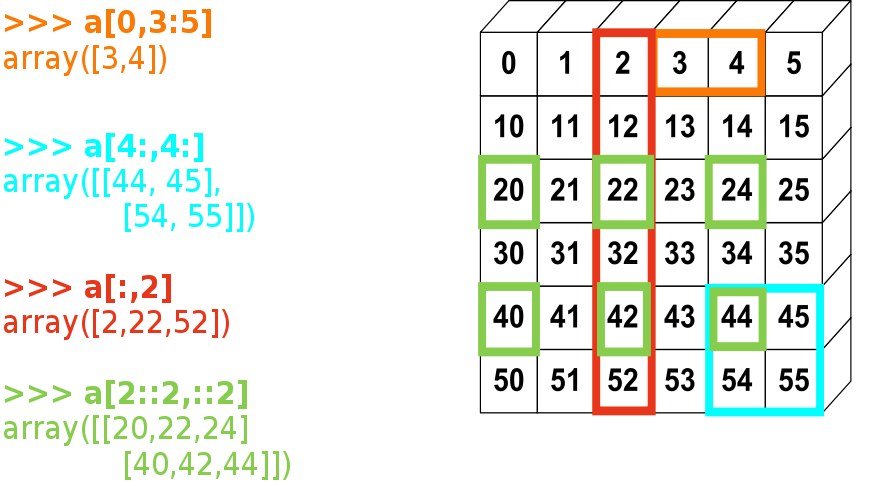
\includegraphics[scale=0.45]{slicing.png}
\end{frame}

\begin{frame}{Scipy/Astropy/PyFITS/SymPy}
  \fontsize{8pt}{8}\selectfont
  \begin{block}{Constants and Conversions}
     For example: \texttt{scipy.constants.c, scipy.constants.hbar, scipy.constants.lambda2nu(550*scipy.constants.nano)}
  \end{block}
  \begin{block}{More Stats}
     Various stats tool using \texttt{scipy.stats}, such as calculating mean, variance, skew, and probability and cumulative density functions
  \end{block}
  \begin{block}{Optimising and Fitting}
      Can use \texttt{scipy.optimize} to find minima (\texttt{.fmin\_bfgs}), find roots of a function (\texttt{.fsolve}), and fitting (\texttt{.curve\_fit})
  \end{block}  
  \begin{block}{PyFits}
      Using \texttt{pyfits}, can import (\texttt{.open()}), read (\texttt{.info()}/\texttt{.header()}), and write (\texttt{.PrimaryHDU()} and \texttt{.writeto()}) FITS files 
  \end{block}  
  \begin{block}{World Coordinate Systems}
      Can find the RA and Dec of pixels using \texttt{astropy.wcs.WCS} and and convert RA and Dec to pixels using \texttt{astropy.wcs.WCS.wcs\_sky2pix()}
  \end{block}
  \begin{block}{Symbolic Calculus}
    Differentiation, Integration, Linear Algebra, Series Expansion, and Equation Simplifying using \texttt{sympy}
  \end{block}
\end{frame}

\begin{frame}{Information on the Web}
  \begin{block}{Documentation}
    \url{http://scipy.org/} \\
    \url{http://matplotlib.org/} \\
    \url{http://www.astropy.org/}
  \end{block}

  \begin{block}{SciPy Tutorials (Also NumPy and Matplotlib)}
    \url{https://conference.scipy.org/scipy2013/tutorials.php}
  \end{block}
  
  \begin{block}{SciPy Lectures (Also NumPy and Matplotlib)}
    \url{http://www.scipy-lectures.org/}
  \end{block}
  
  \begin{block}{Stanford's Introduction to Scientific Python}
    \url{http://web.stanford.edu/~arbenson/cme193.html}
  \end{block}
  
\end{frame}

\begin{frame}{Matplotlib}
  \begin{itemize}
    \item Powerful plotting library. See \url{http://matplotlib.org/gallery.html} for range of examples.
    \item Two interfaces: one similar to MATLAB (for interactive use; relies on global state), and one object-oriented. Typically the latter is to be preferred.
    \item Read the introduction at \url{http://matplotlib.org/faq/usage_faq.html} as this clarifies many points of terminology and usage.
  \end{itemize} 
\end{frame}



% Note that frame must be fragile if we are using lstlisting.
\begin{frame}[fragile]{Matplotlib example}
  \begin{lstlisting}

    import numpy as np
    import matplotlib.pyplot as plt
  
    x = np.arange(0, 2*np.pi, 0.1)
    y = np.sin(x)
  
    plt.figure()
    plt.scatter(x, y) # Or plt.plot...
    plt.show()
  
  \end{lstlisting}
\end{frame}

\begin{frame}[fragile]{Matplotlib Features}
  \fontsize{11pt}{11}\selectfont
  \begin{block}{Different Plotting Styles}
     Can edit marker style, colour, edge colour, size and opaqueness, errorbar style and colour, can annotate plots with text and arrows, and can include colour maps and bars. \\
     Can plot in polar and World Coordinate System coordinates (with the help of \texttt{astropy}).
  \end{block}
  \begin{block}{Image Plotting}
     Can read and plot an image using \texttt{matplotlib.cbook} and \texttt{plt.imshow}
  \end{block}
  \begin{block}{Multiple Subplots}
     Using \texttt{plt.subplot()} you can create multiple subplots, for example the following creates two side-by-side subplots that share x and y axes:\\
     \begin{lstlisting}
plt.subplots_adjust(hspace=0.5)
ax1 = plt.subplot(121)
ax2 = plt.subplot(122, sharex=ax1, sharey=ax1)
     \end{lstlisting}
  \end{block}
\end{frame}


\begin{frame}{Matplotlib exercise}

  \begin{itemize}

  \item Use the SDSS data file (compressed FITS format) \texttt{/share/splinter/ucapwhi/Linux\_training/demo.fits.gz}.
  
  \item Use the pyfits library (\texttt{import astropy.io.fits as pyfits}) to manipulate file columns as numpy arrays.
  
  \item Use the \texttt{open} command to get a handle to the file (\texttt{h = pyfits.open(...)}). Then get e.g. the \texttt{Foo} column via \texttt{x = h[1].data.field[`Foo']}.
  
  \item Create a scatter plot of r-band absolute magnitude (\texttt{`rMAG'}) versus distance (\texttt{`Dist'}). Do you think that this data set is a subset of a larger data set?
  
  \item Make a map by scatter-plotting declination (\texttt{`DEdeg'}) versus right ascension (\texttt{`RAdeg'}). Use small dots. Why is the density lower at the top? Why should the plot really be flipped left/right?
  
  \end{itemize}

\end{frame}


\begin{frame}{Matplotlib exercise - \texttt{BONUS ROUND}}

    \begin{block}{Plot RA versus Dec as an all-sky projection.}
        \fontsize{8pt}{8}\selectfont
        \texttt{HINT}: Use astropy
    \end{block}

\end{frame}  



\begin{frame}{Source control system}

  \begin{itemize}
    \item A source control system is a repository for successive versions of documents (e.g. source code for computer programs).
    \item Versions can be compared and old versions restored if needed (e.g. to undo recent bad changes).
    \item Multiple developers are able to make changes to the same file, with automatic merging of edits from different developers (but if there is an \textit{edit conflict} i.e. two developers change the same line then manual intervention will be needed).
    \item Any serious development that you do (even if just for yourself) should be under the control of a source control system.
  \end{itemize}
\end{frame}
    
\begin{frame}{Git}    
  TODO: Describe Git, draw Git diagram
\end{frame}


\begin{frame}{GitHub and BitBucket}    
  TODO: Describe Github and Bitbucket
\end{frame}




\section{Common Programs}
\begin{frame}{Common and Useful Programs}
  \begin{block}{LaTeX}
    Talk about Tikz in here
  \end{block}
  \begin{block}{DS9}
  \end{block}
  \begin{block}{IRAF}
  \end{block}
  \begin{block}{SExtractor/SWarp}
  \end{block}
\end{frame}

\begin{frame}{DS9}
  \begin{block}{Features}
   \begin{itemize}
    \item{Aligning with WCS (World Coordinate System)}
    \item{Scaling image contrast}
    \item{Funky colour sets (and inverse or negative)}
    \item{Regions and annotating the image}
    \item{Multiple frames; blinking and matching}    
    \item{Contour plots}
  \end{itemize}
  \end{block}
  \begin{block}{DS9 Website}
    \url{http://ds9.si.edu/site/Home.html}
  \end{block}
\end{frame}

\begin{frame}{Image Reduction and Analysis Facility (IRAF)}
  \begin{block}{Features}
   \begin{itemize}
    \item{Uses basic Linux commands to navigate around directories, copy/move files, run tasks in the background}
    \item{A series of packages each containing various tasks}
    \item{\texttt{?} to view all tasks in current package, \texttt{??} to view all tasks}
    \item{Each tasks contains various editable parameter files}
    \item{\texttt{lpar [parameter\_file\_name]} to view and \texttt{epar[parameter\_file\_name]} to edit a  parameter file}    
    \item{\texttt{unlearn [parameter\_file\_name]} to set reset task parameters}
   \end{itemize}
  \end{block}
  \begin{block}{IRAF Websites}
    \url{http://iraf.noao.edu/}\\
    \url{http://iraf.net/irafdocs/}
  \end{block}
\end{frame}

\begin{frame}{SExtractor/SWarp}
  \begin{block}{Features}
   \begin{itemize}
    \item{\textit{''SExtractor is a program that builds a catalogue of objects from an astronomical image. Although it is particularly oriented towards reduction of large scale galaxy-survey data, it can perform reasonably well on moderately crowded star fields.''}}
    \item{\textit{''SWarp is a program that resamples and co-adds together FITS images using any arbitrary astrometric projection defined in the WCS standard.''}}
   \end{itemize}
  \end{block}
  \begin{block}{SExtractor \& SWarp Websites}
    \url{http://www.astromatic.net/software/sextractor}\\
    \url{http://www.astromatic.net/software/swarp}
  \end{block}
\end{frame}

\begin{frame}{CosmoSIS}

\end{frame}

\section{HPC}

\begin{frame}{HPC: Information on the Web}
  \begin{block}{This presentation}
    \url{https://github.com/Astrophysics-UCL/HPCInfo/}
  \end{block}

    \begin{block}{Splinter on the UCL Astrophysics Wiki}
    \url{https://wiki.ucl.ac.uk/display/PhysAstAstPhysGrp/Splinter+User+Guide}
  \end{block}

  \begin{block}{UCL Research Computing Platforms}
    \url{https://wiki.rc.ucl.ac.uk/wiki/Main_Page}
  \end{block}

  \begin{block}{DiRAC}
    \url{http://www.dirac.ac.uk/}
  \end{block}

\end{frame}

\begin{frame}{HPC: Mailing list}
	\url{https://www.mailinglists.ucl.ac.uk/mailman/listinfo/splinter-users}
	\bigskip
	\begin{itemize}
		\item please subscribe
		\item post any issues regarding splinter
	\end{itemize}
\end{frame}

\begin{frame}{HPC: Splinter specs}
	\begin{itemize}
		\item As of \today, \emph{splinter} has 528, 4TB memory
		\item 8 nodes, dual 6-core 2.8GHz, 48GB memory 
		\item 20 nodes, dual 8-core 2.0GHz, 128GB memory
		\item SMP node, 40 2.4GHz cores, 1TB memory
		\item login node, dual 10-core, 2.4GHz 98GB memory
		\item head-node, dual 8-core, 2.4GHz, 164GB memory
	\end{itemize}
\end{frame}

\begin{frame}{HPC: \texttt{splinter} distributed}
  \begin{figure}
    \begin{center}
      \shadowbox{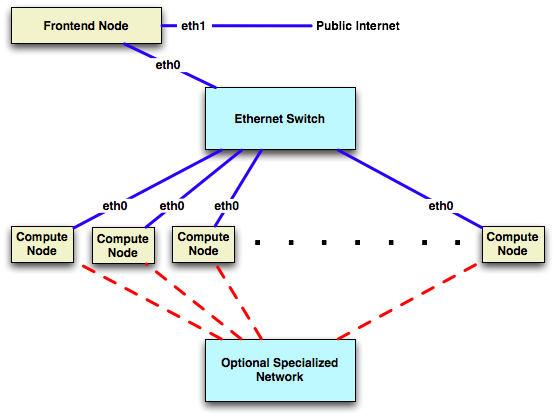
\includegraphics[scale=0.4]{cluster.png}}
      \footnote{\url{http://www.rocksclusters.org/}}
    \end{center}
  \end{figure}
\end{frame}

\begin{frame}{HPC: \texttt{splinter} shared}
  \begin{figure}
    \begin{center}
      \shadowbox{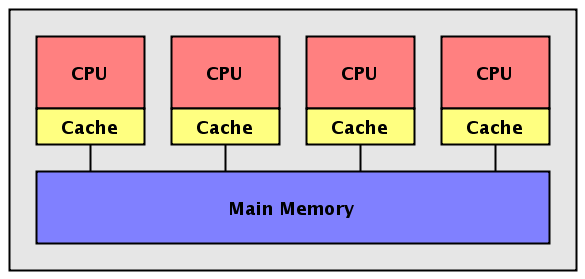
\includegraphics[scale=0.4]{fig03.png}}
      \footnote{\url{http://www.cs.rit.edu/}}
    \end{center}
  \end{figure}
\end{frame}

\begin{frame}{HPC: Workspaces I}
	\begin{block}{\texttt{/home/user\_name}}
		\begin{itemize}
			\item this is your home directory
			\item login scripts can be put here
			\item 1GB quota
			\item private
		\end{itemize}
	\end{block}
	\begin{block}{\texttt{/share/splinter/user\_name}}
		\begin{itemize}
			\item create the directory if not already there
			\item can be used as a workspace
			\item no quota
			\item public unless made private
		\end{itemize}
	\end{block}
\end{frame}

\begin{frame}{HPC: Workspaces II}
	\begin{block}{\texttt{/share/data1}}
		\begin{itemize}
			\item for storing large data
			\item you can create a directory for your, .e.g, \texttt{/share/data1/SKA}
		\end{itemize}
	\end{block}

	\begin{block}{\texttt{/share/apps}}
		\begin{itemize}
			\item for installing software
			\item module-files
		\end{itemize}
	\end{block}
\end{frame}

\begin{frame}{HPC: Login script}
	\begin{itemize}
		\item everytime you login this file will be executed
		\item this file is in your \texttt{\$HOME}
		\item it is called \texttt{.login}
		\item you can load modules, envvars, etc.
	\end{itemize}
	\begin{Examples}
		\begin{block}{Load my aliases}
		    \texttt{source $\sim$/aliases.csh}
                \end{block}
                \begin{block}{Load python}
                     \texttt{module load dev\_tools/nov2014/python-anaconda}
                \end{block}
	\end{Examples}
\end{frame}

\begin{frame}{HPC: Modules}
	\begin{itemize}
		\item easy and flexible way use software
		\item available to everyone in splinter
	\end{itemize}
	
	\begin{Examples}
	    \begin{columns}
                \column{.5\textwidth}
		\begin{block}{Print the available modules}
			\texttt{module avail}
		\end{block}
		\begin{block}{Load a module}
			\texttt{module load module\_name}
		\end{block}
		\begin{block}{List the loaded modules}
			\texttt{module list}
		\end{block}
	
	        \column{.5\textwidth}
		\begin{block}{Unload a module}
			\texttt{module unload module\_name}
		\end{block}
		\begin{block}{Unload all modules}
			\texttt{module purge}
		\end{block}		
		\begin{block}{Help}
			\texttt{module --help}
		\end{block}	
	    \end{columns}								
	\end{Examples}
\end{frame}

\begin{frame}{HPC: Submitting jobs}
	\begin{itemize}
		\item computing jobs should be submitted to the scheduler
		\item you will have to write a job script
		\item interactive job
	\end{itemize}
    \begin{Examples}
	    \begin{columns}
                \column{.5\textwidth}    
		\begin{block}{Submit a job}
			\texttt{qsub job\_script}
		\end{block}
		\begin{block}{Submit an interactive job}
			\texttt{qsub -I}
		\end{block}
		\begin{block}{Check the status of a job}
			\texttt{checkjob job\_id}
		\end{block}

	        \column{.5\textwidth}		
		\begin{block}{List the status of all jobs}
			\texttt{qstat}
		\end{block}
		\begin{block}{Show the queue}
			\texttt{showq}
		\end{block}		
		\begin{block}{Delete a job}
			\texttt{qdel job\_id}
		\end{block}
	    \end{columns}		
    \end{Examples}
\end{frame}

\begin{frame}{HPC: Queues}
	\begin{itemize}
		\item \texttt{compute}
		\item \texttt{cores16}
		\item \texttt{cores12}
		\item \texttt{smp}
	\end{itemize}
\end{frame}

\begin{frame}{HPC: Structure of a job script}
	\texttt{\#!/bin/tcsh \\
	\# PBS -q cores12 \\
	\# PBS -N a\_name\_for\_your\_job \\
	\# PBS -l nodes=1:ppn=6 \\
	\# PBS -l mem=32gb \\
	\# PBS -l walltime=120:00:00} \\
	
	\begin{block}{Set some environment variable}
	    \texttt{setenv OMP\_NUM\_THREADS 6}
        \end{block}
	\begin{block}{Source paths if needed}
	    \texttt{source /home/username/libpaths.csh}
        \end{block}
	\begin{block}{Run my program}
	    \texttt{/home/username/hello\_world.exe}
        \end{block}	
\end{frame}

\begin{frame}{HPC: Jobscripts: things to remember}
	\begin{itemize}
		\item Submit the job to the right queue
		\item Request the correct number of \texttt{nodes} and \texttt{ppn}
		\item Specify the memory required
		\item Always specify the walltime
		\item If your program is not parallel, please use \texttt{nodes=1,ppn=1}
		\item Use \texttt{-q compute} for single processor jobs
		\item Use \texttt{qsub -I} for interactive job
		\item If using most of the resources, please send an email to the mailing list.
	\end{itemize}
\end{frame}

\begin{frame}{HPC: More PBS commands}
	\begin{block}{Specify output}
	    \texttt{PBS -o path/to/file.out}
        \end{block}
	\begin{block}{Specify error output}
	    \texttt{PBS -e path/to/file.err}
        \end{block}
	\begin{block}{Mail alert at (b)eginning, (e)nd, and (a)bortion of execution}
	    \texttt{PBS -m bea}
        \end{block}
	\begin{block}{Send mail to the following address}
	    \texttt{PBS -M your\_email\_id@ucl.ac.uk}
        \end{block}                        
\end{frame}

\begin{frame}{HPC: Using \emph{Ganglia}}
	\url{http://splinter.star.ucl.ac.uk/ganglia/}

	\begin{itemize}
		\item is tool for analysing splinter
		\item can only be loaded from splinter (using firefox)
		\item will give you load/memory information
		\item can look into nodes
	\end{itemize}
\end{frame}

\begin{frame}{HPC: Collaborative projects}
	\begin{itemize}
		\item collaboration between two splinter users
		\item can share common data in \texttt{/share/data1/my\_collaboration}
		\item give read/write permission to other users using \texttt{chmod}
	\end{itemize}
\end{frame}


\begin{frame}{HPC: Best practices}
  \begin{itemize}
    \item Choose the machines that are suited for your problem
    \item Read the User Guide
    \item Do not run your programs in the login node
    \item Install common software locally if and only if absolutely necessary
    \item Request optimum resources
    \item Minimise data transfer between nodes,
    \item \alert{Backup! Backup! Backup!}
  \end{itemize}
\end{frame}

\begin{frame}{HPC: Exercises}
	\url{https://github.com/Astrophysics-UCL/HPCInfo/tree/master/training/workshop_2016/}
\end{frame}

\begin{frame}[fragile]{Extra Slides - Python Examples}
  \fontsize{7pt}{7}\selectfont
  \begin{block}{Dictionary example:}
  \begin{lstlisting}
dc = dict(a=1, b=''Hello World'', c=(1, 2, 3))
print dc.keys(), dc.values(), dc[''b'']
  \end{lstlisting}
  \end{block}
  \begin{block}{Function example:}
  \begin{lstlisting}
def my_first_func(arg1, arg_vol=1, *args, **kwargs):
    print arg1, arg_vol
    for a in args:
        print a
    for key, value in kwargs.iteritems():
        print key, value
  \end{lstlisting}
  \end{block}
  \begin{block}{Class example:}
  \begin{lstlisting}
class my_first_class:
    def __init__(self, arg):
        self.argument = arg

    def print_arg(self):
        return self.argument

instance = my_first_class(42)
print instance.method()
  \end{lstlisting}
  \end{block}
\end{frame}

\begin{frame}[fragile]{Extra Slides - NumPy Examples}
  \fontsize{7pt}{7}\selectfont
  \begin{block}{Shape Manipulation examples:}
  \begin{lstlisting}
a = numpy.arange(60).reshape(6,10)
print a.shape
print a.flatten()
print a.reshape(2, -1, 3)  
  \end{lstlisting}
  \end{block}
  \begin{block}{Sorting examples:}
  \begin{lstlisting}
a = numpy.array([2, 6, 5, 1, 6, 3, 3])
print numpy.sort(a)
print numpy.argsort(a)

data_type = [(''wavelength'', int), (''flux'', float)]
values = [(31, 210), (45, 3400), (18, 150), (7, 50), (21, 100)]
array = numpy.array(values, dtype=data_type)
print numpy.sort(array, order=''wavelength'')
  \end{lstlisting}
  \end{block}
  \begin{block}{I/O examples:}
  \begin{lstlisting}
data = numpy.genfromtxt(file_name, dtype=data_type, 
    delimiter=delimiter_character, skip_header=number_of_lines_to_skip)
data1, data2 = np.loadtxt(file_name, skiprows=number_of_lines_to_skip, 
    unpack=True)
  \end{lstlisting}
  \end{block}
\end{frame}

\begin{frame}[fragile]{Extra Slides - Scipy/Astropy/PyFITS/SymPy Examples 1}
  \fontsize{6pt}{6}\selectfont
  \begin{block}{Constants and conversions example:}
  \begin{lstlisting}
x = scipy.constants.find('Newton')
print scipy.constants.value(x[0]), scipy.constants.unit(x[0])
  \end{lstlisting}
  \end{block}   
  \begin{block}{More stats examples:}
  \begin{lstlisting}
bell = scipy.stats.norm(loc=centre, scale=standard_deviation)
print bell.stats(moments='mvs')
print bell.pdf([value, value_2, value_3])
print bell.cdf([value, value_2, value_3])
  \end{lstlisting}
  \end{block}
  \begin{block}{Optimising and Fitting examples:}
  \begin{lstlisting}
minima1 = scipy.optimize.fmin_bfgs(function, initial_guess)
minima2 = scipy.optimize.brute(function, (search_grid,))

r1 = scipy.optimize.fsolve(function, initial_guess)
r2 = scipy.optimize.newton_krylov(function, initial_guess, verbose=True)

opt_values, covariance_matrix = scipy.optimise.curve_fit(function, x_data, y_data)
plt.plot(x_data, y_data, 'bo', label='data')
plt.plot(x_data, function(x_data, opt_values[0], opt_values[1]), 'r-', label='fit')
  \end{lstlisting}
  \end{block}
\end{frame}

\begin{frame}[fragile]{Extra Slides - Scipy/Astropy/PyFITS/SymPy Examples 2}
  \fontsize{6pt}{6}\selectfont
  \begin{block}{PyFITS examples:}
  \begin{lstlisting}
fh = pyfits.open(file_name)
print fh.info(), fh[1].header()

hdu = pyfits.PrimaryHDU(data)
hdu.writeto(new_image_name, clobber=True) 
  \end{lstlisting}
  \end{block} 
  \begin{block}{World Coordinate System examples:}
  \begin{lstlisting}
wcs = astropy.wcs.WCS(header=pyfits.open(file_name)[1].header)
pixcrd = numpy.array([[coord1_x, coord1_y], [coord2_x, coord2_y]], numpy.float_)
sky = wcs.wcs_pix2sky(pixcrd, 1)
print sky

pixcrd2 = wcs.wcs_sky2pix(sky, 1)
print pixcrd2
  \end{lstlisting}
  \end{block}
  \begin{block}{Symbolic Calculus examples:}
  \begin{lstlisting}
a = sympy.Symbol(''a'')
b = sympy.Symbol(''b'')
e = (a + 2*b)**5
e.diff(b)
sympy.integrate(a**2 * sympy.cos(a), a)
sympy.simplify((a + a*b)/a)
sympy.series(sympy.cos(a), a)
  \end{lstlisting}
  \end{block}
\end{frame}

\begin{frame}[fragile]{Extra Slides - Matplotlib Examples}
  \fontsize{6pt}{6}\selectfont
  \begin{block}{Annotate examples:}
      \url{http://matplotlib.org/examples/pylab_examples/annotation_demo2.html}
  \end{block}
  \begin{block}{Polar and color/size/opaqueness example:}
  \begin{lstlisting}
plt.figure(figsize=(10,10))
ax = plt.subplot(111, polar=True)
c = scatter(angles, radii, c=colors, s=sizes, alpha=opaqueness)
plt.show()
  \end{lstlisting}
  \end{block}
  \begin{block}{Image plot example:}
  \begin{lstlisting}
datafile = matplotlib.cbook.get_sample_data(file_name, asfileobj=True)
A = fromstring(datafile.read(), uint16).astype(float)
A *= 1.0/max(A)
A.shape = 512, 512
im = plt.imshow(A, cmap=cm.hot, origin='upper', extent=plot_size)
plt.show()
  \end{lstlisting}
  \end{block}
  \begin{block}{Subplot and colour bar example:}
  \begin{lstlisting}
fig, axes = plt.subplots(nrows=2, ncols=2)
for dat, ax in zip(data, axes.flat):
    im = ax.imshow(dat, vmin=colour_min, vmax=colour_max)
cax = fig.add_axes([left, bottom, width, height])
fig.colorbar(im, cax=cax)
plt.show()
  \end{lstlisting}
  \end{block}
\end{frame}

\end{document}
